\section{觀念與公式}

\subsection{定義與基本性質}
基於單位圓。\\
\textbf{定義}:
\begin{itemize}
    \item $\sin \theta = y$,$\cos \theta = x$。
    \item $\tan \theta = \frac{\sin \theta}{\cos \theta}$。
\end{itemize}
\textbf{性質}:
\begin{itemize}
    \item 週期:$\sin(\theta + 2\pi) = \sin \theta$。
    \item 奇偶:$\sin(-\theta) = -\sin \theta$,$\cos(-\theta) = \cos \theta$。
\end{itemize}
\textbf{應用}:角度計算。\\
\textbf{大學技巧}:$e^{i\theta} = \cos \theta + i \sin \theta$。

\subsection{三角函數圖形}
波形分析。\\
\textbf{公式}:
\begin{itemize}
    \item $y = A \sin(Bx + C)$:振幅$|A|$,週期$\frac{2\pi}{|B|}$,相位移$-\frac{C}{B}$。
\end{itemize}
\textbf{應用}:週期現象。\\
\textbf{大學技巧}:傅立葉級數。

\subsection{三角恆等式}
基本關係與變換。\\
\textbf{基本公式}:
\begin{itemize}
    \item $\sin^2 \theta + \cos^2 \theta = 1$。
    \item $\sin(\alpha + \beta) = \sin \alpha \cos \beta + \cos \alpha \sin \beta$。
    \item $\cos(\alpha + \beta) = \cos \alpha \cos \beta - \sin \alpha \sin \beta$。
    \item $\sin 2\theta = 2 \sin \theta \cos \theta$。
    \item $\cos 2\theta = 2\cos^2 \theta - 1$。
\end{itemize}
\textbf{積化和差}:
\begin{itemize}
    \item $\sin \alpha \cos \beta = \frac{1}{2} [\sin(\alpha + \beta) + \sin(\alpha - \beta)]$。
    \item $\cos \alpha \sin \beta = \frac{1}{2} [\sin(\alpha + \beta) - \sin(\alpha - \beta)]$。
    \item $\cos \alpha \cos \beta = \frac{1}{2} [\cos(\alpha + \beta) + \cos(\alpha - \beta)]$。
    \item $\sin \alpha \sin \beta = \frac{1}{2} [\cos(\alpha - \beta) - \cos(\alpha + \beta)]$。
\end{itemize}
\textbf{和差化積}:
\begin{itemize}
    \item $\sin \alpha + \sin \beta = 2 \sin\left(\frac{\alpha + \beta}{2}\right) \cos\left(\frac{\alpha - \beta}{2}\right)$。
    \item $\sin \alpha - \sin \beta = 2 \cos\left(\frac{\alpha + \beta}{2}\right) \sin\left(\frac{\alpha - \beta}{2}\right)$。
    \item $\cos \alpha + \cos \beta = 2 \cos\left(\frac{\alpha + \beta}{2}\right) \cos\left(\frac{\alpha - \beta}{2}\right)$。
    \item $\cos \alpha - \cos \beta = -2 \sin\left(\frac{\alpha + \beta}{2}\right) \sin\left(\frac{\alpha - \beta}{2}\right)$。
\end{itemize}
\textbf{應用}:化簡與證明。\\
\textbf{大學技巧}:積分應用。

\subsection{應用與方程}
\textbf{應用}:
\begin{itemize}
    \item 週期運動:$x = A \sin(\omega t)$。
    \item 方程:$\sin x = k$,解$x = \arcsin k + 2n\pi$。
\end{itemize}
\textbf{大學技巧}:反三角函數。

\section{例題解析}

\subsection{例題1:基本性質}
求$\sin 150^\circ$。\\
\textbf{解}:$\sin 150^\circ = \sin(180^\circ - 30^\circ) = \sin 30^\circ = \frac{1}{2}$。

\subsection{例題2:圖形分析}
$y = 2 \sin(3x - \frac{\pi}{2})$,求週期。\\
\textbf{解}:週期$\frac{2\pi}{3}$。

\subsection{例題3:積化和差}
化簡$\sin 60^\circ \cos 30^\circ$。\\
\textbf{解}:$\frac{1}{2} [\sin(60^\circ + 30^\circ) + \sin(60^\circ - 30^\circ)] = \frac{1}{2} [\sin 90^\circ + \sin 30^\circ] = \frac{1}{2} [1 + \frac{1}{2}] = \frac{3}{4}$。

\subsection{例題4:和差化積}
化簡$\sin 75^\circ + \sin 15^\circ$。\\
\textbf{解}:$2 \sin\left(\frac{75^\circ + 15^\circ}{2}\right) \cos\left(\frac{75^\circ - 15^\circ}{2}\right) = 2 \sin 45^\circ \cos 30^\circ = 2 \cdot \frac{\sqrt{2}}{2} \cdot \frac{\sqrt{3}}{2} = \frac{\sqrt{6}}{2}$。

\subsection{例題5:應用題}
波動$y = 3 \cos(2t)$,求最大值。\\
\textbf{解}:最大值$3$。

\section{圖形展示}
$y = \sin x$:
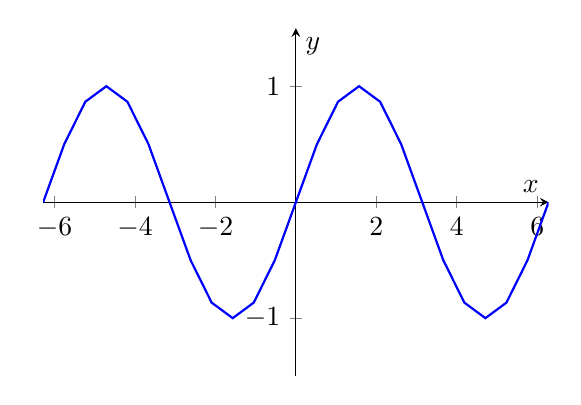
\begin{tikzpicture}
    \begin{axis}[
        axis lines=middle,
        xlabel=$x$,
        ylabel=$y$,
        xmin=-2*pi, xmax=2*pi,
        ymin=-1.5, ymax=1.5,
        width=8cm, height=6cm
    ]
    \addplot[domain=-2*pi:2*pi, blue, thick] {sin(deg(x))};
    \end{axis}
\end{tikzpicture}

\section{題庫}
\begin{enumerate}[label=\arabic*.]
    % 計算題 (10)
    \item 求$\sin 135^\circ$。
    \item 求$\cos 300^\circ$。
    \item $y = 3 \sin(2x)$,求週期。
    \item $\sin 30^\circ \cos 60^\circ$。
    \item $\sin 45^\circ + \sin 15^\circ$。
    \item 求$\cos 120^\circ$。
    \item $y = 2 \cos(4x)$,求振幅。
    \item $\cos 60^\circ \cos 30^\circ$。
    \item $\sin 75^\circ - \sin 15^\circ$。
    \item $\sin \theta \sin 2\theta$,化簡。
    % 應用題 (20)
    \item 求$\sin 105^\circ$。
    \item $y = 4 \sin(3x - \pi)$,求週期。
    \item 化簡$\cos 45^\circ \sin 15^\circ$。
    \item 一波$y = 5 \sin(2t)$,求最大值。
    \item 求$\sin x = \frac{\sqrt{3}}{2}$,$0 \leq x < 2\pi$。
    \item 化簡$\sin 75^\circ + \sin 45^\circ$。
    \item $y = 2 \cos(3x + \frac{\pi}{2})$,求週期。
    \item 化簡$\sin 60^\circ \sin 30^\circ$。
    \item 一物振動$y = 3 \sin(4t)$,求頻率。
    \item 求$\cos 15^\circ - \cos 75^\circ$。
    \item $\cos x = -\frac{1}{2}$,$0 \leq x < 2\pi$。
    \item $y = 5 \sin(2x - \frac{\pi}{4})$,求相位移。
    \item 化簡$\cos 105^\circ + \cos 15^\circ$。
    \item 波動$y = 4 \cos(5t)$,求週期。
    \item 求$\sin 285^\circ$。
    \item $\sin 2\theta \cos \theta$,化簡。
    \item $y = 3 \sin(2x + \pi)$,求振幅。
    \item 化簡$\sin 165^\circ - \sin 105^\circ$。
    \item 一鐘擺$y = 2 \cos(6t)$,求週期。
    \item 求$\sin 45^\circ \cos 15^\circ + \cos 45^\circ \sin 15^\circ$。
    % 觀念題 (10)
    \item 積化和差的用途?
    \item 和差化積如何推導?
    \item 證明$\sin \alpha \cos \beta = \frac{1}{2} [\sin(\alpha + \beta) + \sin(\alpha - \beta)]$。
    \item $\sin^2 \theta + \cos^2 \theta = 1$的意義?
    \item 證明$\sin \alpha + \sin \beta = 2 \sin\left(\frac{\alpha + \beta}{2}\right) \cos\left(\frac{\alpha - \beta}{2}\right)$。
    \item 週期如何定義?
    \item 證明$\cos \alpha \cos \beta = \frac{1}{2} [\cos(\alpha + \beta) + \cos(\alpha - \beta)]$。
    \item 相位移的作用?
    \item 證明$\cos \alpha - \cos \beta = -2 \sin\left(\frac{\alpha + \beta}{2}\right) \sin\left(\frac{\alpha - \beta}{2}\right)$。
    \item 二倍角公式的應用?
    % 進階題 (10)
    \item 化簡$\sin 3\theta \cos \theta$。
    \item $y = 3 \sin(2x) + 4 \cos(2x)$,求振幅。
    \item 化簡$\cos 75^\circ - \cos 15^\circ$。
    \item 求$\cos x = 0$,$0 \leq x < 2\pi$。
    \item $y = 2 \sin(x - \frac{\pi}{3})$,求最小值。
    \item 化簡$\sin 135^\circ + \sin 45^\circ$。
    \item $\sin x + \cos x = 1$,$0 \leq x < 2\pi$。
    \item 化簡$\cos 30^\circ \sin 60^\circ$。
    \item $y = 5 \sin(3x + \frac{\pi}{6})$,求最大值。
    \item 求$\sin 105^\circ \cos 15^\circ$。
    % 挑戰題 (10)
    \item $y = \sin x + \cos x$,求振幅。
    \item 證明$\sin 3\theta = 3 \sin \theta - 4 \sin^3 \theta$。
    \item 化簡$\sin 120^\circ + \sin 60^\circ$。
    \item $y = 4 \sin(2x) - 3 \cos(2x)$,求振幅。
    \item 化簡$\cos 255^\circ - \cos 105^\circ$。
    \item $\sin 2x = \cos x$,$0 \leq x < 2\pi$。
    \item 證明$\cos 2\theta \sin \theta = \frac{1}{2} [\sin 3\theta - \sin \theta]$。
    \item $y = 3 \sin(4x + \frac{\pi}{2})$,求最小值。
    \item 化簡$\sin 75^\circ \cos 45^\circ + \cos 75^\circ \sin 45^\circ$。
    \item 求$\cos 135^\circ + \cos 45^\circ$。
\end{enumerate}